
\documentclass[11pt]{article}
\usepackage[margin=1in]{geometry} 
\usepackage{amsmath,amsthm,amssymb,amsfonts}
\usepackage{listings}
\usepackage{graphicx}
\usepackage{lipsum,calc}
\usepackage[shortlabels]{enumitem}
\usepackage{breqn}
\usepackage{tikz}

\newcommand{\shrug}[1][]{%
\begin{tikzpicture}[baseline,x=0.8\ht\strutbox,y=0.8\ht\strutbox,line width=0.125ex,#1]
\def\arm{(-2.5,0.95) to (-2,0.95) (-1.9,1) to (-1.5,0) (-1.35,0) to (-0.8,0)};
\draw \arm;
\draw[xscale=-1] \arm;
\def\headpart{(0.6,0) arc[start angle=-40, end angle=40,x radius=0.6,y radius=0.8]};
\draw \headpart;
\draw[xscale=-1] \headpart;
\def\eye{(-0.075,0.15) .. controls (0.02,0) .. (0.075,-0.15)};
\draw[shift={(-0.3,0.8)}] \eye;
\draw[shift={(0,0.85)}] \eye;
% draw mouth
\draw (-0.1,0.2) to [out=15,in=-100] (0.4,0.95); 
\end{tikzpicture}}

 
\newcommand{\N}{\mathbb{N}}
\newcommand{\Z}{\mathbb{Z}}

\newenvironment{problem}[2][Problem]{\begin{trivlist}
\item[\hskip \labelsep {\bfseries #1}\hskip \labelsep {\bfseries #2.}]}{\end{trivlist}}

\begin{document}
\title{CSE 574 Homework 3}
\author{Zackary Crosley}
\maketitle

\begin{problem}{1} Markov Decision Processes: Consider the world shown in the figure. Assume that 80\% of the time the agent moves in its intended direction and 10\% of the time it moves in each of the two right angles to that direction. Implement value iteration for each r value below. Discount rewards with a discount factor 0.99. Show the policy obtained in each case and explain why that policy was the intuitive output.
	\begin{equation}
			v^{*} (s) = R(s) + \gamma \max_a \sum_{s'} p(s,a,s') v^{*} (s') \;for\;s = (i,j)\;for\;i, j \in [1, 2, 3]
	\end{equation}
	\begin{verse}
		All values below were generated by the python file value_iteration.py provided.
	\end{verse}
\begin{enumerate}
	\item r = 100
		\begin{itemize}
			\item[Iteration 1]
				\begin{tabular}{l c r}
					189 & 78 & 10 \\
					78 & -1.99 & 6.7 \\
					-1.99 & -1.99 & -1.99 \\
				\end{tabular}
			\item[Iteration 2]
				\begin{tabular}{l c r}
					365.1 & 235.3 & 10 \\
					255.3 & 69.1 & 14.4 \\
					60.58 & -1.99 & 3.55 \\
				\end{tabular}
		\end{itemize}
	\item r = -3
		\begin{itemize}
			\item[Iteration 1]
				\begin{tabular}{l c r}
					-4.2 & 6.722 & 10 \\
					-1.99 & -1.99 & 6.722 \\
					-1.99 & -1.99 & -1.99 \\
				\end{tabular}
			\item[Iteration 2]
				\begin{tabular}{l c r}
					0.257 & 14.4 & 10 \\
					-1.99 & 4.25 & 14.4 \\
					-1.99 & -1.99 & 3.55 \\
				\end{tabular}
		\end{itemize}
	\item r = 0
		\begin{itemize}
			\item[Iteration 1]
				\begin{tabular}{l c r}
					-0.10 & 6.722 & 10 \\
					-1.20 & -1.99 & 6.722 \\
					-1.99 & -1.99 & -1.99 \\
				\end{tabular}
			\item[Iteration 2]
				\begin{tabular}{l c r}
					4.65 & 14.4 & 10 \\
					-1.20 & 4.25 & 14.4 \\
					-1.99 & -1.99 & 3.55 \\
				\end{tabular}
		\end{itemize}
	\item r = 3
		\begin{itemize}
			\item[Iteration 1]
				\begin{tabular}{l c r}
					5.574 & 6.722 & 10 \\
					1.178 & -1.99 & 6.722 \\
					-1.99 & -1.99 & -1.99 \\
				\end{tabular}
			\item[Iteration 2]
				\begin{tabular}{l c r}
					10.35 & 14.4 & 10 \\
					4.96 & 4.45 & 14.4 \\
					-0.41 & -1.99 & 3.55 \\
				\end{tabular}
		\end{itemize}
\end{enumerate}
\end{problem}
\begin{problem}{2} Value Iteration: For the zero-sum, turn-taking game in Homework 2, let R(s) be the reward for A in state s. Let -R(s) be the reward for B with A in state s. Let $U_A (s)$ be the utility of state s when it's A's turn to move in s, and $U_B (s)$ the same for B.
\begin{enumerate}
	\item Write down Bellman equations defining $U_A (s)$ and $U_B (s)$.
		\begin{equation}
			v^{*} (s) = R(s) + \gamma \max_a \sum_{s'} p(s,a,s') v^{*} (s')
		\end{equation}
		\begin{equation}
			U_A (s) = R(s) + \gamma \max_{a_A} \sum_{s'} p(s'|a_A,s) -U_B (s') = R(s) + \gamma \max_{a_A} -U_B (s')
		\end{equation}
		\begin{equation}
			U_B (s) = -R(s)+ \gamma \min_{a_B} \sum_{s'} p(s'|a_B,s) U_A (s') = -R(s) + \gamma \min_{a_B} U_A (s')
		\end{equation}
		\begin{verse}
			$p(s,a,s')$ can be omitted since the probability of moving to intended next state is always 1. Since we only have one s', the $\sum_{s'}$ may also be ommitted. Since unspecified, $\gamma$ will be set to $0.9$.
		\end{verse}
	\item Explain how to do two player value iteration with these conditions and define suitable termination criteria.
		\begin{text}
			States are tuples $(A = [1-4], B = [1-4])$ where $ A \neq B$. May be shortened to simply numbers, so $(A = 1, B = 2) \leftrightarrow (1,2)$
		\end{text}
		\begin{verse}
			Cycle value iterations between positive value iteration from the goal of A and negative value iteration from the goal of B. This is similar to the minimax algorithm in the way it cycles back and forth. Iteration can begin in states that lead to goal nodes, such as (A=3, B=2).
		\end{verse}
	\item Draw the state space showing moves by A in solid lines and moves by B in dashed lines. Mark each state with R(s). Arrange states sA sB on a grid, using sA and sB as coordinates.
		\begin{verse}
			See Figure 1.
		\end{verse}
		\begin{figure}
			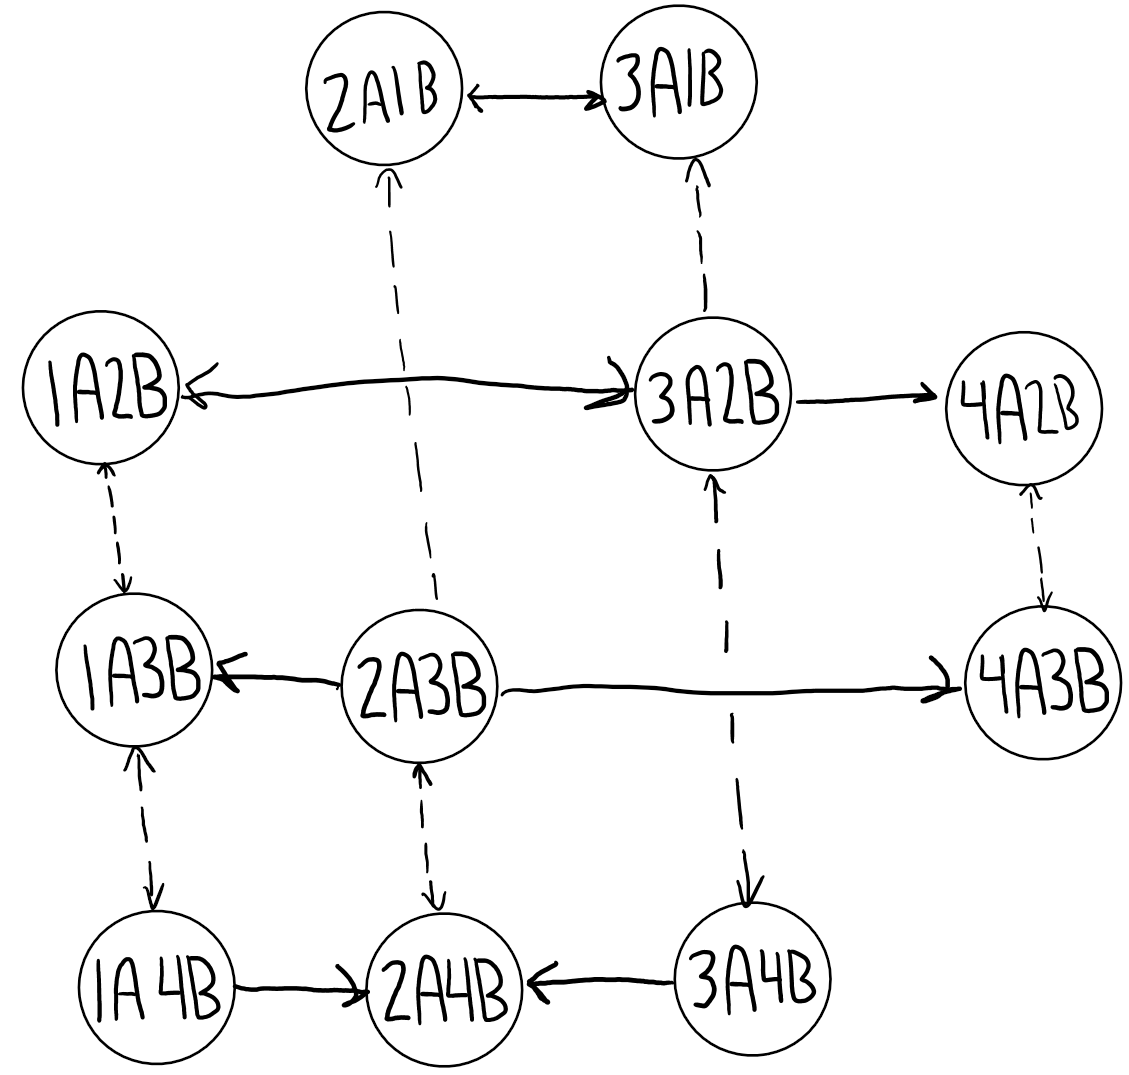
\includegraphics[scale=0.7]{cse545_hw3_p2.PNG}
			\caption{Problem 2c Game State Graph.}
			\label{fig.bfs}
		\end{figure}
	\item Apply two-player value iteration to solve the game, and derive the optimal policy.
		\begin{verse}
			As can be seen in Figure 1, not all states give one or both A and B a choice in move. Any item in position 1 or 4 can only move in one direction, and half those states are win conditions. Only B has a decision in movement in 1A3B; only A has a decision in movement in 2A4B; both have a decision in 2A3B and 3A2B. Thus, these four states are the only ones which require value iteration. Note that the valid movements for the restricted states (excluding the terminal states XA1B and 4AXB, where no movement is valid) are: A right in 1A2B, 1A3B, 1A4B and A left in 3A4B; B left in 1A4B, 2A4B, 3A4B and B right in 1A2B.
		\end{verse}
		\begin{equation}
			R(N,1) = -1; \; R(4,M) = 1; \; R(N,M) = 0 \; where \; N \neq 4 \; and \; M \neq 1 
		\end{equation}
		\begin{itemize}
			\item[(A = 2, B = 3)]
				\begin{equation}
					U_A (s) = R(s) + \gamma \max_{a_A} -U_B (s')
				\end{equation}
				\begin{equation}
					U_A (s) = R((2,3)) + \gamma \max_{a_A} \left[ -U_B ((4,3)), -U_B((1,3)) \right]
				\end{equation}
				\begin{equation}
					U_A (s) = 0 + 0.9 \max_{a_A} \left[ 1, x < 1 \right] = 0.9 \; (Right)
				\end{equation}
				\begin{equation}
					U_B (s) = -R(s) + \gamma \min_{a_B} U_A (s')
				\end{equation}
				\begin{equation}
					U_B (s) = -R((2,3)) + 0.9 \min_{a_B} \left[ U_A ((2,1), U_A(2,4))  \right]
				\end{equation}
				\begin{equation}
					U_B (s) = 0 + 0.9 \min_{a_B} \left[ -1, x > -1)  \right] = -0.9 \; (Left)
				\end{equation}
			\item[(A = 3, B = 2)]
				\begin{equation}
					U_A (s) = R((3,2)) + \gamma \max_{a_A} \left[ -U_B ((4,2)), -U_B((1,2)) \right]
				\end{equation}
				\begin{equation}
					U_A (s) = 0 + 0.9 \max_{a_A} \left[ 1, x < 1 \right] = 0.9 \; (Right)
				\end{equation}
				\begin{equation}
					U_B (s) = -R((3,2)) + 0.9 \min_{a_B} \left[ U_A ((3,1), U_A(3,4))  \right]
				\end{equation}
				\begin{equation}
					U_B (s) = 0 + 0.9 \min_{a_B} \left[ -1, x > -1)  \right] = -0.9 \; (Left)
				\end{equation}
			\item[(A = 2, B = 4)]
				\begin{equation}
					U_A (s) = R((2,4)) + \gamma \max_{a_A} \left[ -U_B ((3,4)), -U_B((1,4)) \right]
				\end{equation}
				\begin{equation}
					U_A (s) = R((2,4)) + \gamma \max_{a_A} \left[ -\left( -0 + \gamma \max_{a_A} 0.9 \right), -\left( -0 + \gamma \max_{a_A} \left[ U_A((1,3)) \right] \right) \right]
				\end{equation}
				\begin{equation}
					U_A (s) = R((2,4)) + \gamma \max_{a_A} \left[ -0.81, 0 \right] = 0 (Left)
				\end{equation}
			\item[(A = 1, B = 3)]
				\begin{equation}
					U_B (s) = -R((1,3)) + 0.9 \min_{a_B} \left[ U_A ((1,2), U_A(1,4))  \right]
				\end{equation}
				\begin{equation}
					U_B (s) = -R((1,3)) + 0.9 \min_{a_B} \left[ \left( R((1,2)) + \gamma \max_{a_A} \left[ -U_B ((3,2)) \right] \right) , \left( R((1,4)) + \gamma \max_{a_A} \left[ -U_B ((2,4)) \right] \right) \right]
				\end{equation}
				\begin{equation}
					U_B (s) = 0.9 \min_{a_B} \left[ \left( 0.9^2 \right) , \left( 0 \right) \right]
				\end{equation}
				\begin{equation}
					U_B (s) = 0 (Right)
				\end{equation}
		\end{itemize}
		\begin{verse}
			Therefore, the optimal policy for A is to move right and B to move left unless that direction is blocked or allows the opponent to jump.
		\end{verse}
\end{enumerate}
\end{problem}
\begin{problem}{3} Suppose we have a machine that is either running or broken down. If it runs throughout one week, it makes a gross profit of \$100. If it fails, the profit is \$0. If it is running at the start of the week and we perform preventive maintenance, the chance it will fail is 0.4. If we do not perform maintenance, the probability is 0.7. Maintenance costs \$20. When the machine is broken, it may be repaired for \$40 with a probability of failure of 0.4 or replaced at a cost of \$150 which is guaranteed to run through its first week. Find the optimal repair, replacement, and maintenance policy for a four week period. Start with a new machine at time 0.
	\begin{verse}
		States: Broken (\$0), Running (\$100)\newline
		Actions: \newline
		Maintain = (Cost: -\$20, 0.4 S+1 = Broken, 0.6 S+1 = Running)\newline
		NoMaintain = (Cost: \$0, 0.7 S+1 = Broken, 0.3 S+1 = Running)\newline
		Repair = (Cost: -\$40, 0.4 S+1 = Broken, 0.6 S+1 = Running)\newline
		Replace = (Cost: -\$150,  1 S+1 = Running)
	\end{verse}
	\begin{equation}
		J_N(x_N) = g_N(x_N)
	\end{equation}
	\begin{equation}
		J_k(x_k) = min_{\mu \in \mu} E_{w_k} \left[ g_k ( x_k, \mu_k, w_k) + J_{k+1} ( f_k ( x_{k+1}, \mu_{k+1}, w_{k+1} ) ) \right]
	\end{equation}
	\begin{itemize}[leftmargin=1in]
		\item[Week 4]
		\begin{dmath}
			v^{*} (Running) = \max_a \left[-20 + (0.4 * 0 + 0.6 * 100), 0 + (0.7 * 0 + 0.3 * 100)\right] = \max_a \left[-20 + 60, 0 + 30\right] = 40 \text{ (Maintain)}
		\end{dmath}
		\begin{dmath}
			v^{*} (Broken) = \max_a \left[-40 + (0.4 \times 0 + 0.6 \times 100), -150 + (1 \times 100)\right] = \max_a \left[-40 + 60, 0 - 50\right] = 20 \text{ (Repair)}
		\end{dmath}
		\item[Week 3]
		\begin{dmath}
			v^{*} (Running) = \max_a \left[-20 + (0.4 \times [0 + 20] + 0.6 \times [100 + 40]), 0 + (0.7 \times [0 + 20] + 0.3 \times [100 + 40])\right] = \max_a \left[-20 + 8 + 84, 14 + 42\right] = 72 \text{ (Maintain)}
		\end{dmath}
		\begin{dmath}
			v^{*} (Broken) = \max_a \left[-40 + (0.4 \times [0 + 20] + 0.6 \times [100 + 40]), (-150 + 1 \times [100 + 40])\right] = \max_a \left[-40 + 8 + 84, -10\right] = 54\text{ (Repair)}
		\end{dmath}
		\item[Week 2]
		\begin{dmath}
			v^{*} (Running) = \max_a \left[-20 + (0.4 \times [0 + 54] + 0.6 \times [100 + 72]), 0 + (0.7 \times [0 + 54] + 0.3 \times [100 + 72])\right] = \max_a \left[-20 + 21.6 + 103.2, 37.8 + 51.4\right] = 104.8\text{ (Maintain)}
		\end{dmath}
		\begin{dmath}
			v^{*} (Broken) = \max_a \left[-40 + (0.4 \times [0 + 54] + 0.6 \times [100 + 72]), (-150 + 1 \times [100 + 72])\right] = \max_a \left[-40 + 21.6 + 103.2, 22\right] = 84.8\text{ (Repair)}
		\end{dmath}
		\item[Week 1]
		\begin{dmath}
			v^{*} (Running) = \max_a \left[-20 + (0.4 \times [0 + 84.8] + 0.6 \times [100 + 104.8]), 0 + (0.7 \times [0 + 84.8] + 0.3 \times [100 + 104.8])\right] = \max_a \left[-20 + 33.92 + 122.88, 59.36 + 61.44\right] = 136.8\text{ (Maintain)}
		\end{dmath}
		\begin{dmath}
			v^{*} (Broken) = \max_a \left[-40 + (0.4 \times [0 + 84.8] + 0.6 \times [100 + 104.8]), (-150 + 1 \times [100 + 104.8])\right] = \max_a \left[-40 + 33.92 + 122.88, 54.8\right] = 116.8\text{ (Repair)}
		\end{dmath}
	\end{itemize}
	\begin{verse}
		Therefore, the optimal policy $\pi^{*}$ is to maintain each week and repair if the machine breaks.
	\end{verse}
\end{problem}
\begin{problem}{4} Dice Blackjack Game - Players bust if they exceed seven they bust. Highest score wins. In event of tie, player two wins. First player roles until they stop, followed by second. Second must roll until at least value 4. Determine stopping strategy for first player when the second player's initial roll is a 3. Hint: Let N = 6 and consider 15 states: 1 busted, 2-8 stopped at sum 1-7, 9-15 at sum 1-7 but still rolling.
	\begin{equation}
		P(win | x^i) = max_{\mu} P(win | x^i)
	\end{equation}
	\begin{equation}
		P(win | x^1) = 0 \; (busted)
	\end{equation}
	\begin{verse}
		Since player 2 must roll to get a 4, starts at 3, and wins on tie, stopped on 4 or less player 1 only wins if player 2 busts.
	\end{verse}
	\begin{equation}
		P(win | x^2) = P(win | x^3) = P(win | x^4 ) = P(win | x^5) = \frac{2}{6} \; (Proability\;p2\;busted)
	\end{equation}
	\begin{verse}
		Player 2 rolls exactly once since he is at 3, stops once he makes or exceeds 4.
	\end{verse}
	\begin{equation}
		P(win | x^6) = P(roll = 1) + p(roll = 5) + p(roll = 6) = \frac{1}{2}
	\end{equation}
	\begin{equation}
		P(win | x^7) = 1 - (P(roll = 3) + p(roll = 4)) = \frac{4}{6}
	\end{equation}
	\begin{equation}
		P(win | x^8) = 1 - p(roll = 4) = \frac{5}{6}
	\end{equation}
	\begin{equation}
		P(win | x^i) \text{for i in [8,15]} = 
	\end{equation}
	\begin{equation}
		J_N(x_N) = g_N(x_N)
	\end{equation}
	\begin{equation}
		J_k(x_k) = min_{\mu \in \mu} E_{w_k} \left[ g_k ( x_k, \mu_k, w_k) + J_{k+1} ( f_k ( x_{k+1}, \mu_{k+1}, w_{k+1} ) ) \right]
	\end{equation}
	\begin{equation}
		J_N(x^i) = p(win | x^i) - (1 - p(win | x^i))
	\end{equation}
	\begin{itemize}
	
	
	
		\item[Roll 7]
		\begin{equation}
			J_N(x^1) = 0 \; \text{(No available actions]}
		\end{equation}
		\begin{equation}
			J_N(x^{15}) = max_{\mu} \left[ \text{Stop:} 1 \times \frac{5}{6}, \text{Roll:} 1 \times 0 \right] = \frac{5}{6} \text{ (Stop)}
		\end{equation}
		
		
		
		\item[Roll 6]
		\begin{equation}
			J_N(x^1) = 0 \; \text{(No available actions]}
		\end{equation}
		\begin{equation}
			J_N(x^{14}) = max_{\mu} \left[ \text{Stop:} 1 \times \frac{4}{6} \text{, Roll:} \frac{5}{6} \times 0 + \frac{1}{6} \times \frac{5}{6}\right] = max_{\mu} \left[ \text{Stop:} \frac{4}{6} \text{, Roll:}\frac{5}{36}\right] =\frac{4}{6} \text{ (Stop)}
		\end{equation}
		\begin{equation}
			J_N(x^{15}) = max_{\mu} \left[ \text{Stop:} 1 \times \frac{5}{6}, \text{Roll:} 1 \times 0 \right] = \frac{5}{6} \text{ (Stop)}
		\end{equation}
		
		
		\item[Roll 5]	
		\begin{equation}
			J_N(x^1) = 0 \; \text{(No available actions]}
		\end{equation}
		\begin{equation}
			J_N(x^{13}) = max_{\mu} \left[ \text{Stop:} 1 \times \frac{3}{6}, \text{Roll:} \frac{1}{6} \times \frac{4}{6} + \frac{1}{6} \times \frac{5}{6} + \frac{4}{6} \times 0 \right] = max_{\mu} \left[ \text{Stop:} \frac{3}{6}, \text{Roll:} \frac{9}{36} \right] = \frac{1}{2} \text{ (Stop)}
		\end{equation}
		\begin{equation}
			J_N(x^{14}) = max_{\mu} \left[ \text{Stop:} 1 \times \frac{4}{6} \text{, Roll:} \frac{5}{6} \times 0 + \frac{1}{6} \times \frac{5}{6}\right] = \frac{4}{6} \text{ (Stop)}
		\end{equation}
		\begin{equation}
			J_N(x^{15}) = max_{\mu} \left[ \text{Stop:} 1 \times \frac{5}{6}, \text{Roll:} 1 \times 0 \right] = \frac{5}{6} \text{ (Stop)}
		\end{equation}
		
		
		
		
		\item[Roll 4]
		\begin{equation}
			J_N(x^1) = 0 \; \text{(No available actions]}
		\end{equation}
		\begin{equation}
			J_N(x^{12}) = max_{\mu} \left[ \text{Stop:} 1 \times \frac{2}{6}, \text{Roll:} \frac{1}{6} \times \frac{4}{6} + \frac{1}{6} \times \frac{5}{6} + \frac{1}{6} \times \frac{1}{2} + \frac{3}{6} \times 0 \right] = max_{\mu} \left[ \text{Stop:} \frac{2}{6}, \text{Roll:} \frac{12}{36}\right] = \frac{2}{6} \text{ (Either)}
		\end{equation}
		\begin{equation}
			J_N(x^{13}) = max_{\mu} \left[ \text{Stop:} 1 \times \frac{3}{6}, \text{Roll:} \frac{1}{6} \times \frac{4}{6} + \frac{1}{6} \times \frac{5}{6} + \frac{4}{6} \times 0 \right] = \frac{1}{2} \text{ (Stop)}
		\end{equation}
		\begin{equation}
			J_N(x^{14}) = max_{\mu} \left[ \text{Stop:} 1 \times \frac{4}{6} \text{, Roll:} \frac{5}{6} \times 0 + \frac{1}{6} \times \frac{5}{6}\right] = \frac{4}{6} \text{ (Stop)}
		\end{equation}
		\begin{equation}
			J_N(x^{15}) = max_{\mu} \left[ \text{Stop:} 1 \times \frac{5}{6}, \text{Roll:} 1 \times 0 \right] = \frac{5}{6} \text{ (Stop)}
		\end{equation}
		
		
		
		\item[Roll 3]	
		\begin{equation}
			J_N(x^1) = 0 \; \text{(No available actions]}
		\end{equation}
		\begin{equation}
			J_N(x^{11}) = max_{\mu} \left[ \text{Stop:} \frac{2}{6}, \text{Roll:} \frac{1}{6} \times \frac{5}{6} + \frac{1}{6} \times \frac{4}{6} + \frac{1}{6} \times \frac{1}{2} + \frac{1}{6} \times \frac{2}{6}\right] = max_{\mu} \left[ \text{Stop:} \frac{2}{6}, \text{Roll:} \frac{14}{36}\right] = \frac{14}{36} \text{ (Roll)}
		\end{equation}
		\begin{equation}
			J_N(x^{12}) = max_{\mu} \left[ \text{Stop:} 1 \times \frac{2}{6}, \text{Roll:} \frac{1}{6} \times \frac{4}{6} + \frac{1}{6} \times \frac{5}{6} + \frac{1}{6} \times \frac{1}{2} + \frac{3}{6} \times 0 \right] = \frac{2}{6} \text{ (Either)}
		\end{equation}
		\begin{equation}
			J_N(x^{13}) = max_{\mu} \left[ \text{Stop:} 1 \times \frac{3}{6}, \text{Roll:} \frac{1}{6} \times \frac{4}{6} + \frac{1}{6} \times \frac{5}{6} + \frac{4}{6} \times 0 \right] = \frac{1}{2} \text{ (Stop)}
		\end{equation}
		\begin{equation}
			J_N(x^{14}) = max_{\mu} \left[ \text{Stop:} 1 \times \frac{4}{6} \text{, Roll:} \frac{5}{6} \times 0 + \frac{1}{6} \times \frac{5}{6}\right] = \frac{4}{6} \text{ (Stop)}
		\end{equation}
		\begin{equation}
			J_N(x^{15}) = max_{\mu} \left[ \text{Stop:} 1 \times \frac{5}{6}, \text{Roll:} 1 \times 0 \right] = \frac{5}{6} \text{ (Stop)}
		\end{equation}
		
		
		
		
		
		
		\item[Roll 2]	
		\begin{equation}
			J_N(x^1) = 0 \; \text{(No available actions]}
		\end{equation}
		\begin{equation}
			J_N(x^{10}) = max_{\mu} \left[ \text{Stop:} \frac{2}{6}, \text{Roll:} \frac{1}{6} \times \frac{5}{6} + \frac{1}{6} \times \frac{4}{6} + \frac{1}{6} \times \frac{1}{2} + 2 \times (\frac{1}{6} \times \frac{2}{6})\right] = max_{\mu} \left[ \text{Stop:} \frac{2}{6}, \text{Roll:} \frac{16}{36}\right] = \frac{16}{36} \text{ (Roll)}
		\end{equation}
		\begin{equation}
			J_N(x^{11}) = max_{\mu} \left[ \text{Stop:} \frac{2}{6}, \text{Roll:} \frac{1}{6} \times \frac{5}{6} + \frac{1}{6} \times \frac{4}{6} + \frac{1}{6} \times \frac{1}{2} + \frac{1}{6} \times \frac{2}{6}\right] = \frac{14}{36} \text{ (Roll)}
		\end{equation}
		\begin{equation}
			J_N(x^{12}) = max_{\mu} \left[ \text{Stop:} 1 \times \frac{2}{6}, \text{Roll:} \frac{1}{6} \times \frac{4}{6} + \frac{1}{6} \times \frac{5}{6} + \frac{1}{6} \times \frac{1}{2} + \frac{3}{6} \times 0 \right] = \frac{2}{6} \text{ (Either)}
		\end{equation}
		\begin{equation}
			J_N(x^{13}) = max_{\mu} \left[ \text{Stop:} 1 \times \frac{3}{6}, \text{Roll:} \frac{1}{6} \times \frac{4}{6} + \frac{1}{6} \times \frac{5}{6} + \frac{4}{6} \times 0 \right] = \frac{1}{2} \text{ (Stop)}
		\end{equation}
		\begin{equation}
			J_N(x^{14}) = max_{\mu} \left[ \text{Stop:} 1 \times \frac{4}{6} \text{, Roll:} \frac{5}{6} \times 0 + \frac{1}{6} \times \frac{5}{6}\right] = \frac{4}{6} \text{ (Stop)}
		\end{equation}
		\begin{equation}
			J_N(x^{15}) = max_{\mu} \left[ \text{Stop:} 1 \times \frac{5}{6}, \text{Roll:} 1 \times 0 \right] = \frac{5}{6} \text{ (Stop)}
		\end{equation}
		
		
		
		
		
		
		\item[Roll 1]	
		\begin{equation}
			J_N(x^1) = 0 \; \text{(No available actions]}
		\end{equation}
		\begin{equation}
			J_N(x^{9}) = max_{\mu} \left[ \text{Stop:} \frac{2}{6}, \text{Roll:} \frac{1}{6} \times \frac{5}{6} + \frac{1}{6} \times \frac{4}{6} + \frac{1}{6} \times \frac{1}{2} + 3 \times (\frac{1}{6} \times \frac{2}{6})\right] = max_{\mu} \left[ \text{Stop:} \frac{2}{6}, \text{Roll:} \frac{18}{36}\right] = \frac{18}{36} \text{ (Roll)}
		\end{equation}
		\begin{equation}
			J_N(x^{10}) = max_{\mu} \left[ \text{Stop:} \frac{2}{6}, \text{Roll:} \frac{1}{6} \times \frac{5}{6} + \frac{1}{6} \times \frac{4}{6} + \frac{1}{6} \times \frac{1}{2} + 2 \times (\frac{1}{6} \times \frac{2}{6})\right] = \frac{16}{36} \text{ (Roll)}
		\end{equation}
		\begin{equation}
			J_N(x^{11}) = max_{\mu} \left[ \text{Stop:} \frac{2}{6}, \text{Roll:} \frac{1}{6} \times \frac{5}{6} + \frac{1}{6} \times \frac{4}{6} + \frac{1}{6} \times \frac{1}{2} + \frac{1}{6} \times \frac{2}{6}\right] = \frac{14}{36} \text{ (Roll)}
		\end{equation}
		\begin{equation}
			J_N(x^{12}) = max_{\mu} \left[ \text{Stop:} 1 \times \frac{2}{6}, \text{Roll:} \frac{1}{6} \times \frac{4}{6} + \frac{1}{6} \times \frac{5}{6} + \frac{1}{6} \times \frac{1}{2} + \frac{3}{6} \times 0 \right] = \frac{2}{6} \text{ (Either)}
		\end{equation}
		\begin{equation}
			J_N(x^{13}) = max_{\mu} \left[ \text{Stop:} 1 \times \frac{3}{6}, \text{Roll:} \frac{1}{6} \times \frac{4}{6} + \frac{1}{6} \times \frac{5}{6} + \frac{4}{6} \times 0 \right] = \frac{1}{2} \text{ (Stop)}
		\end{equation}
		\begin{equation}
			J_N(x^{14}) = max_{\mu} \left[ \text{Stop:} 1 \times \frac{4}{6} \text{, Roll:} \frac{5}{6} \times 0 + \frac{1}{6} \times \frac{5}{6}\right] = \frac{4}{6} \text{ (Stop)}
		\end{equation}
		\begin{equation}
			J_N(x^{15}) = max_{\mu} \left[ \text{Stop:} 1 \times \frac{5}{6}, \text{Roll:} 1 \times 0 \right] = \frac{5}{6} \text{ (Stop)}
		\end{equation}
		
		
		\begin{verse}
			Therefore the optimal policy is to keep rolling below four and stop above four. At four, either stopping or continuing to roll is equally likely to result in a win.
		\end{verse}				
		
	\end{itemize}
\end{problem}
\begin{problem}{5} We are given six coins, one of which is counterfeit and is known to have different weight than the rest. Construct a strategy to find the counterfeit coin using a two-pan scale in a minimum average number of tries. Hint: There are two initial decisions that make sense: (1) test two of the coins against two others, and (2) test one of the coins against one other.
	\begin{verse}
		Obvious strategy is to first compare two coins against two coins. If these are the same weight, then we know the oddly weighted coin is in the remaining two. The first four coins can be marked or separated, depending on what works best. If they are not the same, the unweighed pair of coins must be the normally weighted. Weigh one of the pairs of two coins from the first step against the remaining two. If they are the same, then one of the other two coins must be differently weighted. Else, if they are different, then the pair of coins from the original comparison must contain the oddly weighted coin. We are now down to two coins, one of which must be differently weighted, in at most two comparisons. Weigh one of the remaining coins against a coin which is of known normal weight. If this weight is inequal, then this coin is the counterfeit one. Else, the last coin is. This policy finds the counterfeit coin in two cases, in the best case, and three in the worst.
	\end{verse}
\end{problem}
\begin{problem}{6} In the framework of the basic problem, consider the case where the cost has the multiplicative form:
	\begin{equation}E_{w_{k_{k=0,1,\ldots N-1}}} \left\lbrace g_N (x_N) \times g_{N-1} (x_{N-1}, u_{N-1}, w_{N-1}\ldots g_0(x_0,u_0,w_0) \right\rbrace
	\end{equation}
	\begin{verse}Develop a DP-like algorithm for this problem assuming that $g_k (x_k , u_k , w_k ) \geq 0$ for all $x_k , u_k , w_k$ , and k.
	\end{verse}
	\begin{lstlisting}
		# Assumes x, u, and w are lists of the values for x, u, and w
		# Also assumes function 'g' already exists and handles missing parameters, as 
		#	shown in function.
		E(N, x, u, w):
			ret g(N, x[N]) * g_recursive(N-1, x, u, w)
		
		g_recursive(N, x, u, w):
			ret g(N, x[N], u[N], w[N]) * g_recursive(N-1, x, u, w)
	\end{lstlisting}
\end{problem}
\begin{problem}{7}
	\shrug\
\end{problem}
\end{document}
